\documentclass[12pt,a4paper,openany,oneside]{book}

% 格式控制
%------------------------------------------------------------------------------%
%                                                                              %
%   LaTeX Template for Bachlor Thesis of Northwestern Polytechnical University %
%   Environment Config: TeXLive 2017                                           %
%   * XeTeX 3.14159265-2.6-0.99998 (TeX Live 2017/W32TeX)                      %
%   * BibTeX 0.99d (TeX Live 2017/W32TeX)                                      %
%   Version: 1.5.0.0426                                                        %
%                                                                              %
%------------------------------------------------------------------------------%
%   Copyright by NWPU Metaphysics Office, GPLv3-LICENSE                        %
%------------------------------------------------------------------------------%


%---------------------------------纸张大小设置---------------------------------%
\usepackage{geometry}
% 普通A4格式缩进
% \geometry{left=2.5cm,right=2.5cm,top=2.5cm,bottom=2.5cm}
% 论文标准缩进
\geometry{left=1.25in,right=1.25in,top=1in,bottom=1.5in}
%------------------------------------------------------------------------------%


%----------------------------------必要库支持----------------------------------%
\usepackage{xcolor}
\usepackage{tikz}
\usepackage{layouts}
\usepackage[numbers,sort&compress]{natbib}
\usepackage{clrscode}
\usepackage{gensymb}
\usepackage[final]{pdfpages}
\usepackage{float}
\usepackage{xcolor}
\usepackage{textgreek}
\definecolor{grey}{RGB}{128,128,128}%手动定义灰色,这样就保证了和word的页眉一样
\usepackage{amsmath}
%------------------------------------------------------------------------------%

%--------------------------------设置标题与目录--------------------------------%
\usepackage[sf]{titlesec}
\usepackage{titletoc}
%------------------------------------------------------------------------------%


%--------------------------------添加书签超链接--------------------------------%
\usepackage[unicode=true,colorlinks=false,pdfborder={0 0 0}]{hyperref}
% 在此处修改打开文件操作
\hypersetup{
    bookmarks=true,         % show bookmarks bar?
    pdftoolbar=true,        % show Acrobat’s toolbar?
    pdfmenubar=true,        % show Acrobat’s menu?
    pdffitwindow=true,      % window fit to page when opened
    pdfstartview={FitH},    % fits the width of the page to the window
    pdfnewwindow=true,      % links in new PDF window
}
% 在此处添加文章基础信息
\hypersetup{
    pdftitle={title},
    pdfauthor={author},
    pdfsubject={subject},
    pdfcreator={creator},
    pdfproducer={producer},
    pdfkeywords={key1  key2  key3}
           }
%------------------------------------------------------------------------------%


%---------------------------------设置字体大小---------------------------------%
\usepackage{type1cm}
% 字号与行距,统一前缀s(a.k.a size)
\newcommand{\sChuhao}{\fontsize{42pt}{63pt}\selectfont}                 % 初号, 1.5倍
\newcommand{\sYihao}{\fontsize{26pt}{36pt}\selectfont}                  % 一号, 1.4倍
\newcommand{\sErhao}{\fontsize{22pt}{28pt}\selectfont}                  % 二号, 1.25倍
\newcommand{\sXiaoer}{\fontsize{18pt}{18pt}\selectfont}                 % 小二, 单倍
\newcommand{\sSanhao}{\fontsize{16pt}{24pt}\selectfont}                 % 三号, 1.5倍
\newcommand{\sXiaosan}{\fontsize{15pt}{22pt}\selectfont}                % 小三, 1.5倍
\newcommand{\sSihao}{\fontsize{14pt}{21pt}\selectfont}                  % 四号, 1.5倍
\newcommand{\sHalfXiaosi}{\fontsize{12.5pt}{16.25pt}\selectfont}        % 半小四, 1.25倍
\newcommand{\sLargeHalfXiaosi}{\fontsize{13pt}{19pt}\selectfont}        % 半小四, 1.5倍
\newcommand{\sXiaosi}{\fontsize{12pt}{14.4pt}\selectfont}               % 小四, 1.25倍
\newcommand{\sLargeWuhao}{\fontsize{11pt}{11pt}\selectfont}             % 大五, 单倍
\newcommand{\sWuhao}{\fontsize{10.5pt}{10.5pt}\selectfont}              % 五号, 单倍
\newcommand{\sXiaowu}{\fontsize{9pt}{9pt}\selectfont}                   % 小五, 单倍
%------------------------------------------------------------------------------%


%---------------------------------设置中文字体---------------------------------%
\usepackage{fontspec}
\usepackage[SlantFont,BoldFont,CJKchecksingle]{xeCJK}
\usepackage{CJKnumb}
% 使用 Adobe 字体
\newcommand\adobeSog{Adobe Song Std}
\newcommand\adobeHei{Adobe Heiti Std}
\newcommand\adobeKai{Adobe Kaiti Std}
\newcommand\adobeFag{Adobe Fangsong Std}
\newcommand\codeFont{Consolas}
% 设置字体
\defaultfontfeatures{Mapping=tex-text}
\setCJKmainfont[ItalicFont=\adobeKai, BoldFont=\adobeHei]{\adobeSog}
\setCJKsansfont[ItalicFont=\adobeKai, BoldFont=\adobeHei]{\adobeSog}
\setCJKmonofont{\codeFont}
\setmonofont{\codeFont}
% 设置字体族
\setCJKfamilyfont{song}{\adobeSog}      % 宋体
\setCJKfamilyfont{hei}{\adobeHei}       % 黑体
\setCJKfamilyfont{kai}{\adobeKai}       % 楷体
\setCJKfamilyfont{fang}{\adobeFag}      % 仿宋体
% 用于页眉学校名,特殊字体,powerby https://github.com/ecomfe/fonteditor
\setCJKfamilyfont{nwpu}{nwpuname}
% 新建字体命令,统一前缀f(a.k.a font)
\newcommand{\fSong}{\CJKfamily{song}}
\newcommand{\fHei}{\CJKfamily{hei}}
\newcommand{\fFang}{\CJKfamily{fang}}
\newcommand{\fKai}{\CJKfamily{kai}}
\newcommand{\fNWPU}{\CJKfamily{nwpu}}
%------------------------------------------------------------------------------%


%------------------------------添加插图与表格控制------------------------------%
\usepackage{graphicx}
\usepackage[font=small,labelsep=quad]{caption}
\usepackage{wrapfig}
\usepackage{multirow,makecell}
\usepackage{longtable}
\usepackage{booktabs}
\usepackage{tabularx}
\usepackage{setspace}
%\captionsetup[table]{labelfont=bf,textfont=bf}
\usepackage{ctex}
\let\proofname\relax
\usepackage{setspace}
\usepackage{caption}

% 设置五号黑体字体
\setCJKfamilyfont{songti}{SimSun}
\newcommand*{\myheading}[1]{\multicolumn{1}{c}{\textbf{\heiti\fontsize{9pt}{12pt}\selectfont #1}}}

% 设置表格字体及行距
\renewcommand{\arraystretch}{1.5}
\setlength{\tabcolsep}{8pt}
\setstretch{1.2}

% 设置表格标题格式
\captionsetup[table]{textfont=bf,labelsep=space,labelformat=simple,font={small},skip=0ex}
%------------------------------------------------------------------------------%


%---------------------------------添加列表控制---------------------------------%
\usepackage{enumerate}
\usepackage{enumitem}
%------------------------------------------------------------------------------%


%---------------------------------设置引用格式---------------------------------%
\renewcommand\figureautorefname{图}
\renewcommand\tableautorefname{表}
\renewcommand\equationautorefname{式}
\newcommand\myreference[1]{[\ref{#1}]}
\newcommand\eqrefe[1]{式(\ref{#1})}
% 增加 \ucite 命令使显示的引用为上标形式
\newcommand{\ucite}[1]{$^{\mbox{\scriptsize \cite{#1}}}$}
\renewcommand\arraystretch{1.4}
\renewcommand\theequation{\thesection.\arabic{equation}}
\renewcommand{\thefigure}{\thechapter-\arabic{figure}}
\renewcommand{\thetable}{\thechapter-\arabic{table}}
%------------------------------------------------------------------------------%


%--------------------------------设置定理类环境--------------------------------%
\usepackage[amsthm,thmmarks]{ntheorem}
\newtheorem{myexample}{例}
\newtheorem{thm}{定理}
%------------------------------------------------------------------------------%


%--------------------------设置中文段落缩进与正文版式--------------------------%
\XeTeXlinebreaklocale "zh"                      % 使用中文的换行风格
\XeTeXlinebreakskip = 0pt plus 1pt              % 调整换行逻辑的弹性大小
\usepackage{indentfirst}                        % 段首空格设置
\setlength{\parindent}{26pt}                    % 段首空格长度
\setlength{\parskip}{3pt plus 1pt minus 1pt}    % 段落间距
\renewcommand{\baselinestretch}{1.25}           % 行距
%------------------------------------------------------------------------------%


%----------------------------设置段落标题与目录格式----------------------------%
\setcounter{secnumdepth}{3}
\setcounter{tocdepth}{2}

\newcommand\chapterID[1]{第\CJKnumber{#1}章}
\renewcommand{\chaptername}{第\CJKnumber{\thechapter}章}%今年的模板中的绪论部分“第X章”没有空格,所以把原来这里的“~”删去
\renewcommand{\figurename}{图}
\renewcommand{\tablename}{表}
\renewcommand{\bibname}{参考文献}
\renewcommand{\contentsname}{目~录}
\newcommand{\keywords}[1]{\\ \\ \textbf{关~键~词}:#1}


\titleformat{\chapter}[hang]{\normalfont\sSanhao\filcenter\fHei\bf}%
{\sSanhao{\chaptertitlename}}{20pt}{\sSanhao}
\titleformat{\section}[hang]{\fHei \bf \sXiaosan}%
{\sXiaosan \thesection}{0.5em}{}{}
\titleformat{\subsection}[hang]{\fHei \bf \sLargeHalfXiaosi}%
{\sLargeHalfXiaosi \thesubsection}{0.5em}{}{}
\titleformat{\subsubsection}[hang]{\fHei \bf}%
{(\arabic{subsubsection})}{0.5em}{}{}   % 小标题式的subsubsection:(4) 标题

% 缩小正文中各级标题之间的缩进
\titlespacing{\chapter}{0pt}{-3ex plus .1ex minus .2ex}{0.25em}
\titlespacing{\section}{0pt}{-0.2em}{0em}
\titlespacing{\subsection}{0pt}{0.5em}{0em}
\titlespacing{\subsubsection}{0pt}{0.25em}{0pt}

% 定义目录中各级标题之间的格式以及缩进
\dottedcontents{section}[1.16cm]{}{1.8em}{5pt}
\dottedcontents{subsection}[2.00cm]{}{2.7em}{5pt}
\dottedcontents{subsubsection}[2.86cm]{}{3.4em}{5pt}
\titlecontents{chapter}[0pt]{\fHei\vspace{0.5em}}%
{\contentsmargin{0pt}\fHei\makebox[0pt][l]{\chapterID{\thecontentslabel}}\hspace{3.8em}}%
{\contentsmargin{0pt}\fHei}%
{\titlerule*[.5pc]{.}\contentspage}[\vspace{0em}]
%------------------------------------------------------------------------------%


%---------------------------------设置页眉页脚---------------------------------%
\usepackage{fancyhdr}
\usepackage{fancyref}
%\addtolength{\headsep}{-0.1cm}          %页眉位置
%\addtolength{\footskip}{-0.1cm}         %页脚位置
\addtolength{\topmargin}{0.5cm}
\newcommand{\makeheadrule}{
    \makebox[0pt][l]{\rule[.7\baselineskip]{\headwidth}{0.8pt}}
    \vskip-.8\baselineskip
}
\makeatletter
\renewcommand{\headrule}{%
    {\if@fancyplain\let\headrulewidth\plainheadrulewidth\fi\makeheadrule}}
\pagestyle{fancyplain}
\fancyhf{}
\fancyfoot[C,C]{\sWuhao-~\thepage~-}
% 后续文字可以自行修改
\chead{\sSanhao\raisebox{0.04cm}%
    { \fNWPU 西北工业大学} \fSong{{\textbf{\textcolor{grey}{本科毕业设计论文}} }}}%根据word中的要求改变页眉的颜色
%------------------------------------------------------------------------------%


%----------------------------------其他补充设置--------------------------------%
% 重置列表环境的间隔
% \let\orig@Itemize =\itemize
% \let\orig@Enumerate =\enumerate
% \let\orig@Description =\description

% \def\Myspacing{
%     \itemsep=1.5ex \topsep=-0.5ex \partopsep=0pt \parskip=0pt \parsep=0.5ex
% }

% \def\newitemsep{
%     \renewenvironment{itemize}{\orig@Itemize\Myspacing}{\endlist}
%     \renewenvironment{enumerate}{\orig@Enumerate\Myspacing}{\endlist}
%     \renewenvironment{description}{\orig@Description\Myspacing}{\endlist}
% }

% \def\olditemsep{
%     \renewenvironment{itemize}{\orig@Itemize}{\endlist}
%     \renewenvironment{enumerate}{\orig@Enumerate}{\endlist}
%     \renewenvironment{description}{\orig@Description}{\endlist}
% }

% \newitemsep
% 下划线
\newcommand\dlmu@underline[2][5cm]%
{\hskip1pt\underline{\hb@xt@ #1{\hss#2\hss}}\hskip3pt}
\let\coverunderline\dlmu@underline
%------------------------------------------------------------------------------%


%----------------------------------添加代码控制--------------------------------%
\usepackage{listings}
\lstset{
    basicstyle=\footnotesize\ttfamily,
    numbers=left,
    numberstyle=\tiny,
    numbersep=5pt,
    tabsize=4,
    extendedchars=true,
    breaklines=true,
    keywordstyle=\color{blue}\bfseries,
    numberstyle=\color{purple},
    commentstyle=\color[rgb]{0, 0.4, 0}\bfseries,
    stringstyle=\color{violet}\ttfamily\bfseries,
    rulesepcolor=\color{red!20!green!20!blue!20},
    showspaces=false,
    showtabs=false,
    frame=shadowbox,
    framexrightmargin=5pt,
    framexbottommargin=4pt,
    showstringspaces=false,
    escapeinside=`', %逃逸字符(1左面的键),用于显示中文
}
\renewcommand{\lstlistingname}{CODE}
\lstloadlanguages{% Check Dokumentation for further languages, page 12
    Pascal, C++, Java, Ruby, Python, Matlab, R, Haskell
}
%------------------------------------------------------------------------------%

\endinput
% 这是简单的 thesis(book) 的导言区设置,不能单独编译。


% 非格式控制插件
% \usepackage{math-symbols}
\usepackage{manuals/math-symbols}
% 插图目录
\graphicspath{{figures/}}

% 仅用于测试
\usepackage{blindtext}
%\title{\textsf{比如我举个例子}}
\author{{\kai 谁知道呢}}
\date{May 20, 20xx}
%\numberwithin{equation}{chapter}%公式按章编号
\renewcommand{\theequation}{\thechapter-\arabic{equation}}%公式按章编号,并将编号设置为(1-1)这样的格式

\begin{document}

	\sloppy

	\pagenumbering{Roman}

	% 封皮
	\frontmatter
	% 本科毕业设计论文模板
% 封皮
\begin{titlepage}
    \voffset 2.7cm
    \begin{center}
        \begin{center}
            \begin{minipage}[c]{2.64cm}
                \centering
                \resizebox{!}{0.9cm}{ \parbox{0.54cm}{ \begin{tikzpicture}
    \draw[line width=0.10cm] (0, 0) circle (2.0cm);
    % \fill[gray!15] (0, 0) -- (1.3cm,0cm) arc (0:230:1.3cm) -- cycle;
    % \fill[gray!15] (0, 0) -- (1.3cm,0cm) arc (0:-50:1.3cm) -- cycle;
    \foreach \t in {-50, -40, -30, -20, -10, 0, 10, 20, 30, 40, 50, 60, 70, 80, 90, 100, 110, 120, 130, 140, 150, 160, 170, 180, 190, 200, 210, 220, 230}
    {
        \foreach \p/\d in {0/0.01cm, 5/-0.01cm}
        {
            \foreach \r in {1.27cm, 1.17cm, 1.07cm, 0.97cm}
            {
                \fill (\t + \p: \r + \d) circle (0.01cm);
            }
        }
    };
    \draw[line width=0.03cm] (0, 0) circle (1.32cm);
    \fill[white] (0, 0) circle (0.9cm);
    \draw[line width=0.05cm] (0, 0) circle (0.9cm);
    \fill[black] (-0.50, -0.73) .. controls (-0.35, -0.81) ..
        (-0.2, -0.80) .. controls (0.15, -0.70) and (0.20, -0.60) .. 
        (0.35, -0.35) .. controls (0.42, -0.24) and (0.60, -0.26) ..
        (0.60, -0.40) .. controls (0.58, -0.50) and (0.49, -0.50) ..
        (0.45, -0.45) .. controls (0.40, -0.68) and (0.75, -0.70) ..
        (0.90, 0.00) arc (360:250:0.9cm);
    \fill (-0.40, -0.40)--(-1.33, -0.40)--(1.00, 1.10)--cycle;
    \fill (-0.37, -0.43)--(-0.20, -0.80)--(1.01, 1.05)--cycle;
    
    \foreach \x/\txt in {0/N, 1/O, 2/R, 3/T, 4/H, 5/W, 6/E, 7/S, 8/T, 9/E, 10/R, 11/N, 12/~, 13/P, 14/O, 15/L, 16/Y, 17/T, 18/E, 19/C, 20/H, 21/N, 22/I, 23/C, 24/A, 25/L, 26/~, 27/U, 28/N, 29/I, 30/V, 31/E, 32/R, 33/S, 34/I, 35/T, 36/Y}
    {
        \node[scale=0.7, rotate=\x*-6.50-245] at (207+\x*-6.50:1.6cm) {\txt};
    };

    \foreach \x/\txt in {0/西, 1/北, 2/工, 3/业, 4/大, 5/学}
    {
        \node[scale=1.25, rotate=\x*18-50] at (225+\x*18:1.65cm) {\fNWPU\txt};
    };

    \foreach \x/\txt in {0/1, 1/9, 2/3, 3/8}
    {
        \node[scale=1, rotate=\x*18-25] at (\x*18-115:1.1cm) {\bfseries\txt};
    };
\end{tikzpicture}

\endinput
% 这是西北工业大学校徽文件,不能单独编译。 } }
                \end{minipage}
                \hskip 0.8cm
                \begin{minipage}[c]{8cm}
                \fontsize{33}{33}\fNWPU 西北工业大学
            \end{minipage}
        \end{center}
        \vskip 0.7cm
        \sChuhao\fSong {\bfseries 本科毕业设计论文}
        \vskip 5cm
        \begin{minipage}[c]{18cm} 
        {
        \sSanhao\fHei 题~~目 \hspace{0.7cm}\coverunderline[13.2cm]{壁面粗糙度对水下高速航行器的转捩-湍流特性的影响}%y原来的代码会因为题目过长导致换行,加入mingpage之后解决了问题
        }
        \end{minipage}
        \vskip 1.8cm
        {
            \sSihao\fSong 专业名称\coverunderline[5.5cm]{飞行器设计与工程}
            \vskip 0.7cm
            \sSihao\fSong 学生姓名\coverunderline[5.5cm]{穆宇旸}
            \vskip 0.7cm
            \sSihao\fSong 指导教师\coverunderline[5.5cm]{徐家宽}
            \vskip 0.7cm
            \sSihao\fSong 完成时间\coverunderline[5.5cm]{2023.6.1}
            \vfill
        }
    \end{center}
\end{titlepage}
\fSong \normalsize

\endinput
% 这是封面排版文件,不能单独编译。
	\clearpage 
	\newpage
	\clearpage
	
	
	\setcounter{page}{1}
	\renewcommand{\baselinestretch}{1.25}
	
	% 中文摘要
	\renewcommand{\baselinestretch}{1.5}
\fontsize{12pt}{13pt}\selectfont

\chapter*{摘~~~~要}
\markboth{中~文~摘~要}{中~文~摘~要}

%随着近年来视觉同时定位与地图构建(Visual Simultaneous Localization and Mapping,VSLAM)的快速发展,闭环检测已经成为了移动机器人导航领域的关键问题和研究热点,。闭环检测本质上来说很像一个分类问题,鉴于深度卷积神经网络在图像分类和图像检索任务方面的优越表现,本文提出一种基于卷积神经网络和VLAD的网络模型结构,将该模型作为一种新的视觉SLAM闭环检测方法。

%本文首先对视觉SLAM的研究现状加以介绍,包括基于滤波器和基于图优化的视觉SLAM研究进展。接着详细介绍了作为视觉SLAM重要环节的闭环检测的研究现状,包括基于人工设计特征以及基于深度学习的闭环检测的国内外研究情况。
 
%其次,本文分析了视觉SLAM的基础理论,详细介绍了VSLAM的整体流程。总结了视觉 SLAM 中闭环检测的流程和不同实现方法,对视觉 SLAM 闭环检测的组成模块进行了提炼,并探究了不同模块的现有实现方法及其不足之处。

%接着本文对特征点检测算法进行了研究,分析对比SIFT、SURF和ORB特征描述子方法。针对视觉 SLAM 闭环检测的场景图像描述模块,深入分析了基于传统特征与基于深度学习的图像描述及其存在的问题,然后结合神经网络与 VLAD特征的特性,提出基于融合VGG16网络与NetVLAD特征提取的网络模型框架,介绍了模型的弱监督训练过程及损失函数的计算,给出了实验用的闭环检测方法:用余弦相似度来计算模型提取到的特征向量之间的相似性并构建相似性矩阵,通过比较阈值判断是否构成闭环。

%最后,本文将基于 VGG16-NetVLAD网络模型的闭环检测方法与传统的词袋模型闭环检测方法以及单纯基于VGG16卷积神经网络的闭环检测方法在数据集 New College和City Center上进行了对比实验,对实验结果加以分析,实验结果表明基于VGG16-NetVLAD网络模型在闭环检测上的 PR 性能和特征提取时间性能上具有比较好的表现。

\vspace{-10pt}



\vspace{1em}
\noindent {\fHei 关键词:} \quad %卷积神经网络,闭环检测,视觉同步定位与地图构建,特征提取

\clearpage
\endinput

	% 英文摘要
	\renewcommand{\baselinestretch}{1.5}
\fontsize{12pt}{13pt}\selectfont

\chapter*{Abstract}
\markboth{英~文~摘~要}{英~文~摘~要}

%With the rapid development of Visual Simultaneous Localization and Mapping (VSLAM) in recent years, closed-loop detection has become a key issue and research hotspot in the field of mobile robot navigation. Closed-loop detection is essentially like a classification problem. In view of the superior performance of deep convolutional neural networks in image classification and image retrieval tasks, this paper proposes a network model structure based on convolutional neural networks and VLAD, which is used as a A new visual SLAM closed-loop detection method.

%This article first introduces the research status of visual SLAM, including the research progress of visual SLAM based on filter and graph optimization. Next, the research status of closed-loop detection as an important part of visual SLAM is introduced in detail, including the domestic and foreign research status of closed-loop detection based on artificial design features and deep learning.

%Secondly, this article analyzes the basic theory of visual SLAM and details the overall process of VSLAM. The process and different implementation methods of closed-loop detection in visual SLAM are summarized, the constituent modules of closed-loop detection of visual SLAM are refined, and the existing implementation methods and deficiencies of different modules are explored.

%Then this paper studies the feature point detection algorithm, analyzes and compares the SIFT, SURF and ORB feature descriptor methods. For the scene image description module of visual SLAM closed-loop detection, the image description based on traditional features and deep learning and their existing problems are deeply analyzed, and then combined with the characteristics of neural networks and VLAD features, a feature extraction based on fusion VGG16 network and NetVLAD features is proposed. The network model framework introduces the model's weakly supervised training process and the calculation of the loss function, and gives an experimental closed-loop detection method: using cosine similarity to calculate the similarity between the feature vectors extracted by the model and construct a similarity matrix To determine whether a closed loop is formed by comparing thresholds.

%Finally, this paper compares the closed-loop detection method based on the VGG16-NetVLAD network model with the traditional word-bag model closed-loop detection method and the closed-loop detection method based solely on the VGG16 convolutional neural network on the datasets New College and City Center. The experimental results are analyzed, and the experimental results show that the VGG16-NetVLAD network model has relatively good performance in PR performance and feature extraction time performance in closed-loop detection.



\vspace{1em}
\noindent {\textbf{Key Words:}} \quad% Convolutional Neural Network, Closed loop detection, Visual Simultaneous Localization and Mapping, Feature extraction

\clearpage
\endinput
	
	\renewcommand{\baselinestretch}{1.25}
	\fontsize{12pt}{12pt}\selectfont
	\phantomsection%在目录中正确地添加超链接。如果不加该命令,目录中的某些章节可能无法被正确地点击
	%\tableofcontents%自动生成目录,并且会根据之前定义的标题样式来排版各级标题
	\tableofcontents%自动生成目录,并且会根据之前定义的标题样式来排版各级标题
	\clearpage%命令表示在当前位置开始新页。这个命令通常用于控制页面布局,避免出现奇怪的断页
	
	\mainmatter%命令表示进入正文部分。在此之前的章节编号都是罗马数字,从1开始;在此之后的章节编号都是阿拉伯数字,从1开始。
	
	\renewcommand{\baselinestretch}{1.25}
	\sHalfXiaosi\fSong
	
	% 正文内容
	\chapter{绪论}\label{preface}

\section{研究背景及意义}
水动力噪声是水下高速航行器的主要噪声源。航行器壁面的边界层转捩会使其边界层中层流演变成湍流,在湍流边界层中随机的速度扰动会产生脉动压力,随着这种随机的脉动压力产生的噪声统称为水动力噪声,其强度随航速的增加而迅速增加,辐射声功率正比于航速的5$\sim$7次方 \ucite{俞孟萨2007国外舰船水动力噪声研究进展概述},若不发生空化,边界层噪声是水动力噪声的主要噪声源,其主要由边界层转捩区噪声和湍流边界层噪声构成。既然产生了噪声就有必要对其加以控制,降噪有诸多好处:提高声呐探测精度,进而提高鱼雷命中率和潜艇生存力;减小对内部系统工作的影响;减小阻力,进而降低能耗提高效率,增大航程。水动力噪声的降噪主要通过推迟转捩实现。但水下高速航行器在海水中保持长时间的工作状态航行时,由于电化学腐蚀和海洋寄生物侵蚀等因素往往会形成微粗糙表面,这是影响边界层转捩的重要因素之一,在高速流动条件下,随着粗糙元高度增加,转捩区域明显扩大并有提前的趋势 \ucite{赵云飞2015粗糙物面引起的超声速边界层转捩现象研究}。针对该特征,拟通过毕业设计,构建能够精确预测粗糙度对水下高速航行器表面的转捩-湍流特性影响的预测方法,分析壁面粗糙度对转捩-湍流特性的影响,在本文工作的基础上能够进一步合理优化航行器外形并对转捩致湍流脉动噪声进行控制。


\section{湍流模拟方法概述}
当前主流的湍流的数值模拟方法主要分为三种:直接数值模拟(Direct Numerical Simulation,DNS),大涡模拟(Large Eddy Simulation,LES)及雷诺平均方法(Raynolds averaged Navier-Stocks,RANS)。DNS方法直接求解湍流中所有的涡结构,其最小模拟尺度小于耗散尺度,结果中包含丰富的脉动信息,但随着求解目标的湍流雷诺数增大,最小湍流尺度相对于最大湍流尺度减小,DNS计算所需网格量就会增大,进而使得计算成本大大增加,在工程上仍不具有可实现性。RANS方法对湍流中不同尺度的涡结构进行模化,平均求解所有涡结构信息,对网格分辨率要求较低,忽略了湍流流动的细节,计算精度较低,具有较好的鲁棒性和经济型,可以模拟大部分的简单流动现象,因此在工程上得到了广泛应用。目前广泛使用的湍流模型大多基于RANS方法。Spalart等人 \ucite{spalart1992one}从经验公式和量纲分析法出发,提出了Spalart-Allmaras一方程模型(SA模型),该模型对网格要求不是很高,能较好地处理边界层中粘性区域,但其精度不高,且欠缺对复杂流动进行模拟的能力。在RANS方法发展过程中第一个实用化的两方程模型是Jones等人\ucite{jones1973calculation}提出的$\textkappa-\varepsilon$模型,但其边界条件处理困难,鲁棒性差,不能很好的模拟逆压梯度、流动分离。Wilcox \ucite{wilcox1988reassessment}提出的$\textkappa-\textomega$模型是应用最为广泛的二方程湍流模型之一,其比$\kappa-\varepsilon$模型的鲁棒性更好,便于应用在复杂外形流动中,且能很好的模拟逆压梯度、流动分离,但存在对自由来流条件比较敏感的缺陷。Menter\ucite{menter1993zonal}提出的$\textkappa-\textomega$剪切应力输运模型(Shear Stress Transport,SST)在近壁面区采用$\textkappa-\textomega$模型,在边界层外缘和自由剪切区使用$\textkappa-\varepsilon$模型,并通过Bradshaw假设(边界层中剪切应力正比于湍动能)引入了雷诺剪切应力输运的影响。其吸收了$\textkappa-\varepsilon$模型、$\textkappa-\textomega$模型、JK模型的优点,该模型能很好预测逆压梯度和流动分离,以其适用性广、精度高、鲁棒性好的优势成为了应用最为广泛的湍流模型之一。LES方法则介于DNS方法和RANS方法之间,由Smagorinsky \ucite{smagorinsky1963general}最早提出:将小尺度的涡模化,降低了在高雷诺数流动时使用DNS方法计算带来的高计算成本;对大尺度的涡直接求解,捕捉到使用RANS方法时难以预测的涡分离流动,弥补了使用RANS方法在计算复杂流动时精度不高的问题。但LES方法在近壁处存在缺陷:在近壁面的湍流流动中,有着大量脉动尺度正比于壁面距离的小尺度的湍流脉动,随着雷诺数增大,湍流尺度变小,为了求解壁面域需要设置大量网格点,进而带来巨大计算量。
\section{转捩预测方法概述}
在转捩预测方法上,基于RANS的转捩模型具有较好的精度、鲁棒性和经济性,因此被大量用于工程中。基于RANS方法的转捩模型是主要的转捩预测方法,其虽然无法捕捉到足够的脉动信息,但计算量较小且预测精度较高,所需变量能当地化求解,兼有可以与现代大型CFD求解器兼容的优点。在转捩模型研究的最初期,Wilcox 等人 \ucite{wilcox1998turbulence, wilcox1993turbulence}发现低雷诺数湍流模型具有预测转捩的能力,但既没有考虑转捩的间歇现象,也没有考虑层流动能;Dhawan和 Narasimha \ucite{narasimha1985laminar, dhawan1958some}最早根据平板边界层实验给出了间歇因子 的经验关系式。而后众多学者们基于拟合公式构造出$\gamma$输运方程,比较有代表性的有Steelant和Dick  \ucite{steelant2001modeling}基于Dhawan和Narasimha的经验公式 \ucite{narasimha1985laminar, dhawan1958some}构造出的$\gamma$输运方程。但间歇因子只描述转捩过程,为了预测转捩还需要转捩起始位置判据,这一判据通常基于动量厚度雷诺数$Re_\theta$发展而来,在层流流场中一旦超过由经验确定的临界值,即认为发生转捩。Menter和Langtry \ucite{langtry2006correlation, menter2005transition, langtry2009correlation}基于大量实验数据拟合了转捩动量厚度雷诺数的经验公式,并使用涡量雷诺数$Re_\upsilon$替代动量厚度雷诺数$Re_\theta$进行当地化求解,提出了$\gamma-\overline{Re_\theta}$转捩模型。该模型所有变量均可当地化求解,与现代CFD技术兼容,具有大规模并行计算的能力。研究人员们针对基于$\textkappa-\omega~SST$湍流模型的$\gamma-\overline{Re_\theta}$转捩模型在水下航行器表面的转捩预测方面也进行了诸多探索。Rahman等人 \ucite{rahman2022capturing}对$SST~\gamma-\overline{Re_\theta}$转捩模型进行了修正,修改了混合函数$F_2$,并引入了应力-强度参数作为涡流与层流粘度比$R_T$的函数。结果表明该模型能很好预测低雷诺数水翼的边界层转捩现象。Delafin等人 \ucite{delafin2014effect}研究了层流分离泡诱导转捩对水翼升力、阻力和力矩系数的影响,结果表明$SST~\gamma-\overline{Re_\theta}$转捩模型在中等雷诺数条件下能很好地捕捉水翼表面的转捩现象。Ye等人 \ucite{ye2021improvement}通过对$SST~\gamma-\overline{Re_\theta}$转捩模型中的转捩起始雷诺数$Re_{{\theta}t}$进行修正,提高了该模型对弯曲水翼边界层转捩的预测精度
\section{粗糙表面模拟方法概述}
众多研究人员们针对壁面粗糙度问题对湍流模型进行了修正。考虑壁面粗糙度的湍流模型修正重要方法之一是等效沙砾法,在工程中有着广泛的应用。Nikuradse在其1933年的粗糙管道实验 \ucite{nikuradse1950laws}中首次提出等效沙砾法的概念,即通过沙砾高度描述表面粗糙度,并将沙砾高度作为新参数导入模型,进而增强壁面湍流。在此基础上,研究人员们针对各个湍流模型提出了不同的修正方法。Durbin等人\ucite{2001Rough}通过引入流体动力学粗糙度长度,并修改边界条件以在完全粗糙和完全光滑之间进行插值,为两层 模型建立了一个粗糙壁模型。Aupoix等人 \ucite{aupoix2003extensions}将一方程Spalart-Allmaras(SA)湍流模型用于粗糙壁面,根据壁面涡粘度和粗糙高度之间关系进行方程的修正。Knoop等人 \ucite{knopp2009new}提出了可用于$\textkappa-\omega~SST$模型的粗糙壁面公式,对壁面湍动能和比耗散率进行修正。建立在考虑壁面粗糙度对湍流模型进行修正的基础上,研究人员们进一步考虑表面粗糙度对边界层转捩模型进行修正: Ge等人 \ucite{ge2015intermittency}使用了有效原点对光滑表面转捩模型的壁距离进行修改,该原点取决于等效沙砾粗糙度。该模型能够根据转捩位置和粗糙度高度、雷诺数和入口湍流强度预测转捩开始。Dassler \ucite{dassler2010transport}等人引入了新的变量粗糙增长因子$A_r$到$\gamma-\overline{Re_\theta}$转捩模型中,$A_r$的值取决于壁面上的等效沙砾粗糙度高度,会通过附加的转运方程在流场中对流并耗散。通过$A_r$输运方程和$Re_{{\theta}t}$输运方程的相互作用,使得$Re_{{\theta}t}$减小,转捩位置提前。Langel等人 \ucite{langel2015further}通过加入粗糙增长因子$A_r$来扩充Langtry-Menter转捩模型,该额外的变量和输运方程允许将表面粗糙度的非当地影响传递到粗糙段下游,该模型还引入了局部压力梯度的影响和粗糙度密度变化进行修正。Yang等人 \ucite{yang2019distributed}提出了四方程$\textkappa-\omega-\gamma-A_r$转捩模型,从指定壁面上的边界条件中的对流和扩散获得$A_r$的空间分布,$A_r$的作用是放大有效长度尺度,这导致放大了第一模态时间尺度,从而导致更早的转捩,同时提出了对第一模态时间尺度的修改,以明确反应湍流强度(Tu)的影响。Liu等人 \ucite{liu2020predicting}基于层流动能转捩模型(${{\textkappa}_T}-{{\textkappa}_L}-{\omega}模型$)建立了四方程层流动能转捩模型,将粗糙度放大因子的附加输运方程与层流动能转捩模型相结合,再通过粗糙度放大因子修改有效长度尺度,以放大第一模态和第二模态的特征时间尺度。此外为了模拟全湍流区的粗糙度效应,修正了特定湍流耗散率的壁面边界条件。Zhang等人 \ucite{zhang2022modeling}提出了一种结合粗糙度放大因子输运方程的间歇转捩模型,以预测粗糙表面上转捩的开始。将粗糙度修正应用于壁边界条件,对具有不同粗糙表面的平板和涡轮叶片的预测结果与实验数据吻合良好。
\section{本文主要工作安排} 
本毕业设计研究的目的是构建能够精确预测粗糙度对水下高速航行器表面的转捩-湍流特性影响的预测方法,研究壁面粗糙度对转捩-湍流特性的影响。

本文工作安排如下:

第一章~引言。~说明研究背景,研究目标和研究意义,并介绍国内外的研究现状。

第二章~转捩-湍流预测方法。~介绍$SST~\gamma-\overline{Re_\theta}$转捩模型,并通过平板算例、S809风力机翼型算例和NLF0416翼型算例来验证使用该转捩模型能够准确预测转捩现象。

第三章~考虑粗糙壁面的转捩预测方法。~首先介绍耦合$A_r$输运方程的$SST~\gamma-\overline{Re_\theta}$转捩模型,第一步是介绍粗糙因子$A_r$输运方程,接下来说明如何将粗糙度影响耦合在$\gamma-\overline{Re_\theta}$转捩模型上。最后通过粗糙平板算例、粗糙NACA0012翼型和粗糙S814翼型来验证使用耦合$A_r$输运方程的$SST~\gamma-\overline{Re_\theta}$转捩模型能够准确预测粗糙转捩现象。

第四章~水下航行器粗糙转捩特性分析。~本次毕业设计的目标是构建能够精确预测粗糙度对水下高速航行器表面的转捩-湍流特性影响的预测方法,因此基于以上章节的粗糙转捩模型,需要进行对水下航行器粗糙转捩特性进行分析,针对suboff潜艇和鱼雷在不同的实验状态下进行分析。

第五章~总结与展望。~针对本文工作进行总结,说明本文工作中需要进一步改善的问题,并对未来可以继续深入研究的方向进行展望。

\clearpage
\endinput
	%\newpage
%\mbox{}
%\newpage
\chapter{转捩-湍流预测方法}\label{introduction}
\section{$SST~\gamma-\overline{Re_\theta}$转捩模型概述}


 
%\begin{equation}
%\mequlist{x_k=f(x_{k-1},u_k,w_k) \\ z_{k,j}=h(y_j,x_k,w_{k,j})}
%\label{eqn_slam_theory}
%\end{equation}

\section{转捩模型算例验证}
%闭环检测是视觉 SLAM 的重要组成部分,经过前端视觉里程计计算相邻帧数据、后端进行状态最优估计之后,所得到的数据直接用于构造地图会有明显误差,因为视觉里程计对摄像机的初始运动估计存在误差并随着时间的进行产生累积误差,无法构建全局一致的轨迹和地图。如图 \ref{fig_without_loopclose}和图 \ref{fig_with_loopclose}所示,闭环检测算法会对全局地图增加一个约束关系,使得机器人生成的地图更加准确。
\subsection{无压力梯度平板}

\subsection{有压力梯度平板}

\subsection{S809风力机}

\subsection{Nlf(1)-0416}

%\begin{figure}[htbp]
%	\centering
%	\includegraphics[scale=0.6]{figures/chap2-without closed-loop detection.png}
%	\caption{未经闭环检测}
%	\label{fig_without_loopclose}
%\end{figure}

%\begin{figure}[htbp]
	%\centering
	%\includegraphics[scale=0.6]{figures/chap2-with closed-loop detection.png}
	%\caption{经过闭环检测修正后}
	%\label{fig_with_loopclose}
%\end{figure}

%\subsection{闭环检测过程}
%闭环检测的核心问题主要有图像特征的提取与描述、视觉场景建模、图像检索和图像间相似性度量四个部分,其流程图如下所示:

%\begin{figure}[ht]
%	\centering
%	\includegraphics[scale=0.6]{figures/chap2- closed-loop detection.png}
%	\caption{闭环检测流程图}
%\end{figure}




 
 \section{本章小结}
%本章阐述了视觉 SLAM 闭环检测的相关原理和方法。首先,叙述了视觉 SLAM 的基础理论,并着重介绍了视觉 SLAM 闭环检测的实现方法和组成模块。其次,对基于场景外观的闭环检测方法的场景图像描述、闭环决策模型等模块的传统方法存在的不足进行了探讨,为后续深入研究做好铺垫。

\clearpage
\endinput

	
\chapter{考虑粗糙壁面的转捩预测方法}
根据第二章中对$SST~\gamma-\overline{Re_\theta}$转捩模型的介绍和实际算例计算,说明了使用该模型计算转捩时能较好的模拟bypass转捩
 
\section{表面粗糙度模型介绍}
\subsection{粗糙增长因子$A_r$输运方程}
\subsection{边界条件修正}
\subsection{耦合转捩模型}

\section{粗糙转捩模型算例验证}
本节通过对分离零压力梯度粗糙平板,顺、逆压力梯度粗糙平板,粗糙NACA0012翼型和粗糙S814翼型这三个算例中表面粗糙度对转捩的影响进行分析,进而对耦合$A_r$输运方程的$SST~\gamma-\overline{Re_\theta}$粗糙转捩模型的预测水平进行检验。
\subsection{粗糙平板算例}
本小节选用Fenindt的粗糙平板实验 \ucite{feindt1957untersuchungen}作为验证算例,该实验最早被Dassler等人\ucite{dassler2010modelling}用来进行模型的验证。Feindt\ucite{feindt1957untersuchungen}设置了不同压力梯度来研究粗糙高度和转捩位置的关系。在使用粗糙转捩模型进行数值模拟时,保持入口高度$h_0$和平板长度$L$固定,除了零压力梯度算例外,顺、逆压力梯度算例通过设置上壁面的形状来形成收缩-扩张管道来实现。非零压力梯度的上表面轮廓通过函数$h(x)$确定:
\begin{equation} \label{roughnessupper}
h(x)=\frac{{h_0}^2}{\sqrt{1.0-PG}}
\end{equation}
在该表达式中,参数$PG$设置为于Feindt\ucite{feindt1957untersuchungen}实验中两个非零压力梯度测试的条件相匹配。入口高度$h_0$设置为$0.1495L$,以匹配Dassler等人的原始CFD算例中的网格。由Dassler等人\ucite{dassler2010modelling}模拟的压力梯度可知压力梯度参数$PG$设置如下:
\begin{equation}
PG = \left\{ \begin{array}{rcl}
0.458x& \mbox{逆压梯度}
\\-0.430x & \mbox{顺压梯度}
\end{array}\right.
\label{PG参数设置}
\end{equation}
式中$x$为平板流向距离,平板长度$L$设置为1m,根据根据公式\autoref{roughnessupper}和 \ref{PG参数设置},可以得到粗糙平板计算域的上边界轮廓,网格分布如图3-1、3-2和3-3所示。三套网格在边界层上第一层无量纲化网格高度$y^+$均小于1。
\begin{figure}[htbp]
	\centering
	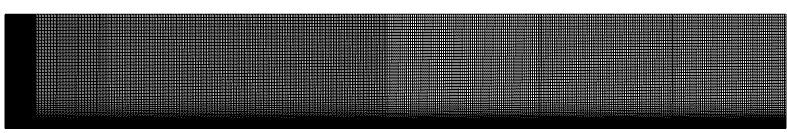
\includegraphics[scale=1]{figures/zero_mesh.jpg}
	\caption{无压力梯度平板}
\end{figure}
\begin{figure}[htbp]
	\centering
	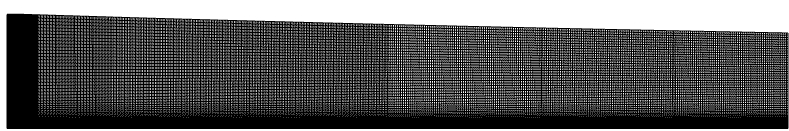
\includegraphics[scale=1]{figures/favorable_mesh.png}
	\caption{顺压力梯度平板}
\end{figure}
\begin{figure}[htbp]
	\centering
	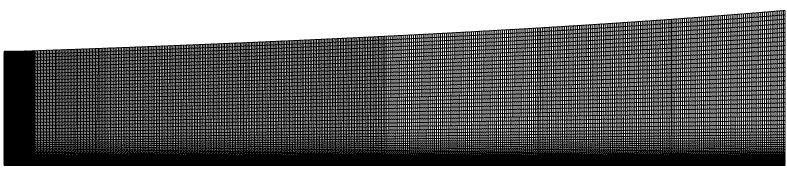
\includegraphics[scale=1]{figures/adverse_mesh.png}
	\caption{逆压力梯度平板}
\end{figure}
在计算边界条件设置上,入口马赫数为0.2。自由来流湍流度为$1.0\%$,基于平板长度的雷诺数设置为$1.3\times10^6$。根据以上设置对从$0\mu m$到$257\mu m$的八个不同粗糙高度的平板进行计算,对于不考虑粗糙度影响的壁面$k_s=0\mu m$具体的边界条件设置如表3-1所示。
\begin{table}[htbp]
	\centering
	\caption{粗糙平板计算条件}
	\label{tab:my_label}
	\begin{tabular}{|>{\centering\arraybackslash}p{1.5cm}|>{\centering\arraybackslash}p{1.5cm}|>{\centering\arraybackslash}p{1.5cm}|>{\centering\arraybackslash}p{5cm}|} % 每列的宽度可以根据需要进行调整
		\hline
		$M_a$ & $R_e$ & $T_u\%$ &  $k_s(\mu m)$ \\ \hline
		0.2 & $1.3\times10^6$ & 1.5 & 0,40,120,193,220,275  \\ \hline
	\end{tabular}
\end{table}

为了观察粗糙度对平板边界层转捩的影响,由于表面表面摩擦力系数$C_f$能直观地反映出转捩位置,应当从$C_f$入手观察。如图3-4所示,该图展示了表面摩擦系数$C_f$受粗糙高度的影响,可以清晰地看出随着$k_s$的增加,无压力梯度粗糙平板上的转捩位置不断提前。


\subsection{粗糙NACA0012翼型}
\subsection{粗糙S814翼型}





\section{本章小结}


\clearpage
\endinput

	%\chapter{基于融合CNN与VLAD的网络模型}
如上文所述,基于深度学习的图像描述方法对动态场景具有更好的鲁棒性,但神经网络在生成全局图像描述的过程中破坏了图像的局部空间特性,对闭环检测的准确率有很大的影响,因此对神经网络的输出进行相关的处理,保留图像的空间特征非常有必要。鉴于基于传统特征的图像描述方法能够有效的保存图像的局部特性,并且基于 VLAD 方法没有损失信息,比 BoVW 对局部信息的刻画更加细致。基于这些特性,本文构建融合 VGG16 和 VLAD 的网络模型 VGG-NetVLAD,使用 VLAD 对 CNN 提取的图像特征进行编码,结合 CNN 提取抽象特征信息的能力与 VLAD 无量化损失的特性,致力于提高图像描述在闭环检测中的准确性与鲁棒性。

\begin{figure}[htbp]
	\centering
	\includegraphics[scale=0.5]{figures/chap4-flow chart.png}
	\caption{基于CNN与VLAD融合的图像描述生成流程}
\end{figure}

\section{基于CNN的图像特征提取}
VGG \ucite{Szegedy2014Going}模型是2014年于 ILSVRC 竞赛中提出的深度卷积神经网络,包含11到19层等不同深度的网络结构,相比于 AlexNet 神经网络,VGG 神经网络结构简单,其使用连续堆叠的小卷积核代替大卷积核以增加网络深度,增强了网络的表达能力,在提升了网络性能的同时减少了网络参数。VGG 中根据卷积核大小和卷积层数目的不同,可分为A,A-LRN,B,C,D,E共6种配置(ConvNet Configuration),其中D,E两种配置较为常用,分别称为 VGG16 和 VGG19。

\begin{figure}[H]
	\centering
	\includegraphics[scale=0.5]{figures/chap4-vgg.png}
	\caption{VGG结构配置}
	\label{vgg_con}
\end{figure}

\subsection{VGG16网络结构}
上图中,每一列对应一种结构配置。例如,图中绿色部分即指明了 VGG16 所采用的结构。我们针对 VGG16 进行具体分析发现,VGG16 共包含:

\begin{itemize}
\item13个卷积层(Convolutional Layer),分别用conv3-XXX表示

\item3个全连接层(Fully connected Layer),分别用FC-XXXX表示

\item5个池化层(Pool layer),分别用maxpool表示
\end{itemize}

其中,卷积层和全连接层具有权重系数,因此也被称为权重层,总数目为13+3=16,这即是
VGG16 中16的来源。(池化层不涉及权重,因此不属于权重层,不被计数)。

\begin{figure}[H]
	\centering
	\includegraphics[scale=0.8]{figures/chap4-vgg16.png}
	\caption{VGG16 模型网络结构}
\end{figure}
 
\subsection{VGG16分块结构}
我们注意图 \ref{vgg_con}右侧,VGG16 的卷积层和池化层可以划分为不同的块(Block),从前到后依次编号为Block1~block5。每一个块内包含若干卷积层和一个池化层。例如:Block4包含:

•3个卷积层,conv3-512

•1个池化层,maxpool

并且同一块内,卷积层的通道(channel)数是相同的,例如:

•block2中包含2个卷积层,每个卷积层用conv3-128表示,即卷积核为:3x3x3,通道数都是128

•block3中包含3个卷积层,每个卷积层用conv3-256表示,即卷积核为:3x3x3,通道数都是256

\begin{figure}[htbp]
	\centering
	\includegraphics[scale=0.3]{figures/chap4-vgg16 block.png}
	\caption{按照块划分的VGG16的结构图}
\end{figure} 

\subsection{VGG16权重参数}
VGG的输入图像是 224x224x3 的图像张量(tensor),随着层数的增加,后一个块内的张量相比于前一个块内的张量:

•通道数翻倍,由64依次增加到128,再到256,直至512保持不变,不再翻倍

•高和宽变减半,由 224→112→56→28→14→7

尽管VGG的结构简单,但是所包含的权重数目却达到了139,357,544个参数。这些参数包括卷积核权重和全连接层权重。

•例如,对于第一层卷积,由于输入图的通道数是3,网络必须学习大小为3x3,通道数为3的的卷积核,这样的卷积核有64个,因此总共有(3×3×3)x64 = 1728个参数。

•计算全连接层的权重参数数目的方法为:前一层节点数×本层的节点数前一层节点数×本层的节点数。因此,全连接层的参数分别为:

o	7x7x512x4096 = 1027,645,444

o	4096x4096 = 16,781,321

o	4096x1000 = 4096000

\begin{figure}[htbp]
	\centering
	\includegraphics[scale=0.6]{figures/chap4-vgg16 weights.png}
	\caption{VGG16网络参数计算过程(不考虑偏置)}
\end{figure}

图中蓝色是计算权重参数数量的部分;红色是计算所需存储容量的部分。

\subsection{VGG16优势及缺陷}
VGG16的突出特点是简单,体现在:

1.卷积层均采用相同的卷积核参数

卷积层均表示为conv3-XXX,其中conv3说明该卷积层采用的卷积核的尺寸(kernel size)是3,即宽(width)和高(height)均为3,$3\times3$是很小的卷积核尺寸,结合其它参数(布幅stride=1,填充方式padding=same),这样就能够使得每一个卷积层(张量)与前一层(张量)保持相同的宽和高。XXX代表卷积层的通道数。

2.池化层均采用相同的池化核参数

池化层的参数均为2××2,步幅stride=2,max的池化方式,这样就能够使得每一个池化层(张量)的宽和高是前一层(张量)的1212。

3.模型是由若干卷积层和池化层堆叠(stack)的方式构成,比较容易形成较深的网络结构。

由于VGG16具有庞大的参数数目,故具有很高的拟合能力;但同时缺点也很明显:

1.即训练时间过长,调参难度大。

2.需要的存储容量大,不利于部署。


\section{基于VLAD的特征编码}
NetVLAD \ucite{Arandjelovic2017NetVLAD}是于2016年提出的一种场景识别算法,该算法改进于 VLAD,VLAD 算法以 SIFT 或该类算法为基础,对其提取的特征进行编码,得到一段较短的特征串,NetVLAD 以卷积神经网络作为基础特征提取结构,与该网络连接,实现端到端的训练。

\subsection{VLAD公式的可微化}
由上文已知VLAD 的主要流程如下:

- 对图像x的全部$N \times D$维局部特征进行 K-Means 聚类获得K个聚类中心,记为$c_k$
- 找到每个聚类中心中的所有的$X$,然后以该聚类中心为基础,计算所有的残差和:遍历所有的样本点,利用$a(x)$决定是否属于该样本点,然后计算相应的残差,最后求和,这样得到了一个聚类中心的残差和,得到$V$的一行。遍历k个聚类中心,得到$V$的k行。通过以下公式将$N \times D$维局部特征编写为一个全局特征$V$,特征向量维数为$K \times D$,其中$k\in K$,$j\in D$,公式如下:

\begin{equation}
V(j, k) = \sum_{i=1}^N a_k(x_i)( x_i(j) - c_k(j) )
\end{equation}

其中$x_i$为第i个局部图像特征,$C_k$为第k个聚类中心,$x_i(j)$和$C_k(j)$分别代表第i个特征向量和第k个聚类中心的第j个元素,$a_k(x_i)$表示第i个特征向量对应第k个聚类中心的权重,当该特征属于这个聚类中心时,权重为1,否则为0。

由于$a_k(x_i)\in\left\{0,1\right\}$,无法利用神经网络进行训练,所以 NetVLAD 层采用了一种近似的方式,将$a_k{x_i}$软分配到多个聚类中心,使其可微:

\begin{equation}
\bar{a}_k(x_i) = \frac{e^{-\alpha\left\|x_i-c_k\right\|^2}}{\sum_{k'}e^{-\alpha\left\|x_i-c_{k'}\right\|^2}}
\end{equation}

其中$\alpha$是一个正值参数,控制响应随距离大小的衰减;显然当$\alpha \to \infty$时,$\bar{a}_k(x_i)$更趋近于0和1的两级。再将 $-\alpha\left\|{x_i-c_k}\right\|^2$展开,显然$e^{-\alpha\left\|{x_i}\right\|^2}$可以被约掉,因此得到: 

\begin{equation}
\bar{a}_k(x_i) = \frac{e^{2\alpha c_k x_i-\alpha\left\|c_k\right\|^2}}{\sum_{k'}e^{2\alpha c_{k'} x_i-\alpha\left\|c_{k'}\right\|^2}} 
\end{equation}

在此令$w_k=2\alpha c_k$,$b_k=-\alpha\left\|c_k\right\|^2$,将其化为一个 softmax 函数。这样原 VLAD 公式就被改写为:   

\begin{equation}
V(j, k) = \sum_{i=1}^N \frac{e^{W_k^{T}x_i+b_k}}{\sum_{k'}e^{W_{k'}^{T}x_i+b_{k'}}}( x_i(j) - c_k(j) )
\end{equation} 

公式中$ {w_k} $、$ {b_k} $和$ {c_k} $都是 NetVLAD 需要训练的参数。原始VLAD中只有一个参数$ {c_k} $,这使得NetVLAD相对于传统的方法具有更加的灵活性,并且所有的参数在特定的任务下可以通过端到端的方式来训练得到。

\subsection{NetVLAD网络实现} 

\begin{figure}[htbp]
	\centering
	\includegraphics[scale=0.4]{figures/chap4-netvlad.png}
	\caption{NetVLAD网络结构}
\end{figure} 
 
首先,由于是 NN 的方法,故使用 CNN Feature 代替了传统 VLAD 中的 N 个局部描述子,CNN是一个全局的特征,它的 Feature Map 是$W \times H \times D$大小,那么类比于我们之前的传统方法$N \times D$, NetVLAD 目标就是将$W \times H \times D$($N=W \times H$)的特征转换为 $K \times D$的特征;其次,将整个 NetVLAD 看做一个 pooling layer,它的作用是实现降最终和 VLAD 一样获得我们想要的$K \times D$维描述子。 
 
\begin{figure}[H]
	\centering
	\includegraphics[scale=0.8]{figures/chap4-netvlad layer.png}
	\caption{NetVLAD网络实现步骤}
	\label{netvlad step}
\end{figure} 
如图 \ref{netvlad step}所示,具体实现分步骤进行:

1. soft-assignment阶段的整个过程可以公式化为一个soft-max函数$ (\sigma_k (z)=\frac{e^{z_k}}{\sum_{{k}'} e^{z_{k'}}}) $,它可以视为分为两个阶段:

- 用K个$1 \times 1$的卷积核卷积矩阵,卷积矩阵参数为$ {w_k} $,偏置项为$ {b_k} $,产生结果$ s_k(x_i)=w_K^{T}+b_k $

- 将上一步的结果送入$ \sigma_k $求得soft-assignment$ \bar{a}_k(x_i) $; 

3. 实现$(x_i (j)- c_k(j))$,也就是公式中的绿色部分,这部分就是一个减法,直接用一个 VLAD core完成;
  
4. 1~3已经实现了$V(j,k)$的计算,后面对 $V(j,k)$做两步简单的归一化(归一化可以提升检索性能),包括:

-  intra-normalization

将每一个 VLAD block(即每个聚类中心的所有残差)分别进行L2归一化,并将矩阵V转换成向量。

-  L2 normalization

对第一步得到的向量整体进行一次L2归一化,最后输出的特征向量维度为$K \times D$。

\section{VGG16-NetVLAD网络模型的框架}

\begin{figure}[H]
	\centering
	\includegraphics[scale=0.6]{figures/chap4-vgg-netvlad.png}
	\caption{VGG16-NetVLAD网络模型}
\end{figure} 

原VGG16模型是一个多层神经网络,主要由3层类型组成:5个卷积层(conv1,conv2,conv3,conv4,conv5),5个最大池化层(pool1,pool2,pool3,pool4,pool5)和3个完全连接的层(fc6,fc7,fc8). 最大池化层为相关特征提供平移不变性并同时减小其尺寸. 事实上,它也是通过合并底层本地信息来构建抽象表示的过程. 而对于完全连接层,前一层中的所有神经元都完全连接到当前层的每个单个神经元. 全连接层主要应用在神经网络的高层网络中,这是因为其有利于图像分类和图像检索应用.

输入层是一幅224×224×3的三通道图像,卷积层和全连接层的激活函数均采用修正线性单元(Rectified Linear Unit, ReLU). ReLU是目前使用最多的激活函数,主要因为其收敛更快,并且能保持同样效果. 标准的ReLU函数为

\begin{equation}
f(x) = max(x,0)
\end{equation}

当$x>0$时,输出$x$ ;当$x \leq 0$时,输出为0。 

ReLU 模块如图 \ref{relu_mod}所示

\begin{figure}[htbp]
	\centering
	\includegraphics[scale=0.4]{figures/chap4-RELU.png}
	\caption{ReLU 模块示意图}
	\label{relu_mod}
\end{figure}

原 VGG 网络输出的结果为图像的分类,不适合用于图像特征的表达。相比于层次更深维度更低的全连接层,全连接层之前的池化层更加适用于视觉闭环检测。池化层同时保留输入图像的大部分空间信息和丰富的语义表示,而全连接层失去了绝大部分空间信息只保留了图像高阶语义信息。

因此对VGG16网络进行了裁剪,去掉了最后一个卷积层conv5-3之后的池化层和全连接层,包括RELU激活函数,并将NetVLAD层连接到卷积层conv5-3之后,作为新的池化层,并将其输出作为图像的全局特征描述符。NetVLAD层将VLAD的思想引入到了卷积神经网络中,构建新的网络模型VGG-NetVLAD。


\section{VGG16-NetVLAD网络模型的训练}
为了训练本文提出的NetVLAD网络,需要解决两个主要的问题:

1.怎么聚合足够多的标注训练数据来训练网络?
 
2.如何得到一个合适的损失函数?

为了解决这两个方法,首先将使用具有极大数量的谷歌时光机(Google Street View Time Machine)弱标签全景图像集作为VGG16-NetVLAD网络的训练集。另外,设计了一个新的弱监督排序损失函数用于处理数据集中不完整和具有噪声的位置信息标注。

\subsection{弱监督性数据集}
采用Google Street View Time Machine弱标签全景图像集训练构建的网络模型,获得最优参数$ {w_k} $、$ {b_k} $和$ {c_k} $。数据集中图片为全景图,每个全景图由一组不同方向的透视图组成,每个透视图只有代表其在地图上大致位置的 GPS 标签,属于弱监督信息。

\begin{figure}[H]
	\centering
	\includegraphics[scale=0.4]{figures/chap4-Google Street View Time Machine.png}
	\caption{谷歌街景时光机例图}
\end{figure}
 
每一列显示在不同时间从附近位置的全景图生成的透视图图像。利用这些图像资源来训练网络,使其学会不受视点和照明(a-c)和适当的遮挡(b)等变化的影响。该图像数据集还可训练网络抑制令人困惑的视觉信息,例如云(a),车辆和人(b-c),并选择忽略植被或学习季节不变的植被表示(a - c)。
该新颖的数据源对于学习用于位置识别的图像表示是宝贵的。像上图所示,相同的位置在不同的时间和季节被描绘,为学习算法提供了关键信息,该算法可以用来发现哪些特征是有用的或令人分心的,以及图像表示应该对哪些变化保持不变,以便获得良好的位置识别性能。

该图像数据集的缺点是它只能提供不完整和嘈杂的监督。每个Time Machine全景图都带有一个GPS标签,只给出它在地图上的大致位置,可以用来识别附近的全景图,但不提供所描绘的场景部分之间的对应关系。具体来说,由于测试查询是来自照相手机的透视图像,所以每个全景图由在不同方向和两个仰角上均匀采样的一组透视图像表示。每个透视图像都标有源全景图的GPS位置。因此,两个地理上接近的透视图像不一定描绘相同的对象,因为它们可能面对不同的方向或可能发生遮挡(例如,两个图像彼此相距一角)。

\subsection{NetVLAD通过监督学习获得聚类中心的好处}

\begin{figure}[htbp]
	\centering
	\includegraphics[scale=0.8]{figures/chap4-Training Cluster Center.png}
	\caption{监督训练VLAD的优势}
	\label{tra_adv}
\end{figure} 
将$c_k$作为学习参数的优点通过图 \ref{tra_adv}可得到直观显示:
  
传统 VLAD 的中心是聚类出来的,没有监督的标签数据 ckVLAD ,在聚类时我们使用了很多图像,这些图像的描述符之间没有关系,那么也就很可能把本来不是一个物体的描述符聚为一类,使得原本期望的类内描述符都是一个物体的特征不太容易达到。而在使用监督数据进行训练时,已知图像数据属于同一物体,那么训练时就可以只把属于同一物体的特征聚在一起而把不是的划分到其他类别,这样就可能学习出一个更好的ckNetVLAD聚类中心,使得最终的特征更有区分度。

\subsection{弱监督排序损失函数}
通过弱监督三元组排序损失算法(triplet ranking loss)来处理谷歌街景时光机图像位置标注的不完整和噪声。将整个网络看做一个特征提取函数$F_\theta$ ,训练目标为:给定一个查询图像q,要在数据集所有图像$I_i$中找到与q位置距离最近的图像$I_i*$。数据集根据GPS信息将与其距离相近(10米以内)的图像作为正样本集合$\left\{p_i^q\right\}$,距离很远(超过25米)的图像作为负样本集合$\left\{n_j^q\right\}$, 构建一个新的三元组数据集(q,$\left\{p_i^q\right\}$,$\left\{n_j^q\right\}$), 在三元组中,正样本$\left\{p_i^q\right\}$中至少包含一幅能与查询图像匹配的图像。训练每一个三元组时,要学习一种最优的图像表示方法$f_\theta$使得查询图像q与最佳匹配图像$\left\{p_{i*}^q\right\}$的距离小于查询图像q与任何一个负样本图像的距离:

\begin{equation}
\mathrm { d } \theta(q,p_{i*}^q)< \mathrm { d } \theta(q,n_j^q),\forall j
\end{equation}

并且正样本中距离最近的应该就是我们想要的最近图片:

\begin{equation}
p_i*^q = \mathop{\arg\min}_{p_i^q}\mathrm { d } \theta(q,p_i^q)
\end{equation}

据此构造如下损失函数( loss):

\begin{equation}
L_\theta = \sum_{j} l(\mathop {\min}\mathrm { d } ^2 \theta(q,p_i^q)+m-\mathrm { d } ^2 \theta(q,p_i^q))
\end{equation}

其中l为hinge loss函数:l(x)=max(x,0),m为附加常数,是一个常量表示给负样本设置的差额(margin)。$L_\theta$代表所有负样本图像的损失之和,对于每一个负样本图像,当其与查询图像的距离大于查询与最佳匹配图像的距离与m之和,则损失为0,否则其损失值与m成正比。通过采用随机梯度下降法对参数进行优化,使网络可提取最优的图像表达。

\section{本章小结}
结合上一章的分析,提出了融合 CNN 与 VLAD 特征的图像描述方法,搭建 VGG16-NetVLAD 卷积神经网络模型的框架,并对构成网络模型的VGG16网络以及NetVLAD层进行了详细介绍,然后介绍了模型的训练方法及得出损失函数的计算过程。

\clearpage
\endinput

	%\chapter{全文总结}
视觉 SLAM 作为移动机器人各种应用的基础以及自动驾驶、VR、AR 等应用的重要组成部分受到了极大的关注,是移动机器人视觉导航中的核心问题之一。闭环检测作为视觉 SLAM 的重要环节,是机器人判断自己当前位置是否位于已访问过的环境区域,成功检测出闭环,可以显著地减小前端视觉里程计的累积误差,并以此作为地图是否需要更新校正的依据,决定着机器人定位的精度与地图构建的一致性,然而由于传统算法的局限性,目前的闭环检测算法仅仅能有效的应对小范围的静态室内环境。鉴于现实场景的复杂性,本文针对闭环检测过程中的场景图像描述、闭环决策模型等模块进行了深入系统的研究,结合深度学习在图像分类与检索任务中的优异性与传统方法的实用性,提出了基于融合 CNN 与 VLAD 特征的图像描述。

本文完成的主要工作总结如下:

1.查阅大量国内外文献资料,分析了移动机器人视觉导航中的视觉 SLAM 问题,概述了视觉 SLAM 和闭环检测的研究现状,重点阐述了现有闭环检测方法存在的问题。

2.通过对视觉 SLAM 的基础理论的分析以及对视觉 SLAM 闭环检测不同实现方法的总结,对视觉 SLAM 闭环检测的组成模块进行了提炼,并探究了不同模块的现有实现方法及其不足之处。

3.比较了 SIFT、SURF 和 ORB 这三种特征点算法的优缺点,针对视觉 SLAM 闭环检测的场景图像描述模块,深入分析了基于传统特征与基于深度学习的图像描述及其存在的问题,然后结合神经网络与 VLAD特征的特性,提出基于融合 CNN 与 VLAD 特征的图像描述方法。

4.
详细介绍了 VGG16-NetVLAD 卷积神经网络模型的框架,然后介绍了模型的训练参数的设置,然后给出了实验用的闭环检测方法,用余弦相似度来计算两特征向量之间的相似性,最后在标准的闭环检测数据集 New College 和City Center上进行测试,分别和几种传统基于人工设计特征的方法(BoVW)以及其他几种深度学习模型的方法进行了对比验证,实验结果表明本文采用的VGG16-NetVLAD 卷积神经网络模型在闭环检测的 PR 性能和特征提取时间性能上具有比较好的优势,为视觉 SLAM 闭环检测提供了一种新方法。

本文只对一些方面做出了研究,仍有许多问题有待于进一步研究与完善,具体包括以下几个方面: 

1.对于主流的传统人工特征方法在特征提取与描述子计算方面要尝试使用更新更快的算法进一步提高闭环检测算法的效率。 

2.要设计更加精简、快速而又对于闭环检测效果比较好的深度模型,本文用的模型虽然效果比较好,但是训练时间长,提取特征文件所占资源也较大,因此更高配置的计算机资源也是必要。

3.本文采用对比验证试验还略显不够,没有考虑光照等条件变化对各种算法能否成功检测出闭环的影响的对比,后续尝试增加对该方面试验进行验证。同时目前算法在复杂光照条件下进行的闭环检测准确度较低,解决这一问题可帮助视觉 SLAM 技术得到更加广泛的应用,提升视觉 SLAM 技术的普及程度。

4. 深度学习方法与视觉 SLAM 技术结合的其他场景应需继续研究,传统视觉 SLAM 只能生成传统的地图,而与深度学习结合,可以生成语义地图,使得机器人完成更复杂的功能来满足人们的需求。


\endinput
	%\chapter{全文总结}
视觉 SLAM 作为移动机器人各种应用的基础以及自动驾驶、VR、AR 等应用的重要组成部分受到了极大的关注,是移动机器人视觉导航中的核心问题之一。闭环检测作为视觉 SLAM 的重要环节,是机器人判断自己当前位置是否位于已访问过的环境区域,成功检测出闭环,可以显著地减小前端视觉里程计的累积误差,并以此作为地图是否需要更新校正的依据,决定着机器人定位的精度与地图构建的一致性,然而由于传统算法的局限性,目前的闭环检测算法仅仅能有效的应对小范围的静态室内环境。鉴于现实场景的复杂性,本文针对闭环检测过程中的场景图像描述、闭环决策模型等模块进行了深入系统的研究,结合深度学习在图像分类与检索任务中的优异性与传统方法的实用性,提出了基于融合 CNN 与 VLAD 特征的图像描述。

本文完成的主要工作总结如下:

1.查阅大量国内外文献资料,分析了移动机器人视觉导航中的视觉 SLAM 问题,概述了视觉 SLAM 和闭环检测的研究现状,重点阐述了现有闭环检测方法存在的问题。

2.通过对视觉 SLAM 的基础理论的分析以及对视觉 SLAM 闭环检测不同实现方法的总结,对视觉 SLAM 闭环检测的组成模块进行了提炼,并探究了不同模块的现有实现方法及其不足之处。

3.比较了 SIFT、SURF 和 ORB 这三种特征点算法的优缺点,针对视觉 SLAM 闭环检测的场景图像描述模块,深入分析了基于传统特征与基于深度学习的图像描述及其存在的问题,然后结合神经网络与 VLAD特征的特性,提出基于融合 CNN 与 VLAD 特征的图像描述方法。

4.
详细介绍了 VGG16-NetVLAD 卷积神经网络模型的框架,然后介绍了模型的训练参数的设置,然后给出了实验用的闭环检测方法,用余弦相似度来计算两特征向量之间的相似性,最后在标准的闭环检测数据集 New College 和City Center上进行测试,分别和几种传统基于人工设计特征的方法(BoVW)以及其他几种深度学习模型的方法进行了对比验证,实验结果表明本文采用的VGG16-NetVLAD 卷积神经网络模型在闭环检测的 PR 性能和特征提取时间性能上具有比较好的优势,为视觉 SLAM 闭环检测提供了一种新方法。

本文只对一些方面做出了研究,仍有许多问题有待于进一步研究与完善,具体包括以下几个方面: 

1.对于主流的传统人工特征方法在特征提取与描述子计算方面要尝试使用更新更快的算法进一步提高闭环检测算法的效率。 

2.要设计更加精简、快速而又对于闭环检测效果比较好的深度模型,本文用的模型虽然效果比较好,但是训练时间长,提取特征文件所占资源也较大,因此更高配置的计算机资源也是必要。

3.本文采用对比验证试验还略显不够,没有考虑光照等条件变化对各种算法能否成功检测出闭环的影响的对比,后续尝试增加对该方面试验进行验证。同时目前算法在复杂光照条件下进行的闭环检测准确度较低,解决这一问题可帮助视觉 SLAM 技术得到更加广泛的应用,提升视觉 SLAM 技术的普及程度。

4. 深度学习方法与视觉 SLAM 技术结合的其他场景应需继续研究,传统视觉 SLAM 只能生成传统的地图,而与深度学习结合,可以生成语义地图,使得机器人完成更复杂的功能来满足人们的需求。


\endinput
	% 参考文献设置
	\clearpage
	\phantomsection
	\addcontentsline{toc}{chapter}{\fHei 参考文献}
	\sXiaosi
	% npu专用
	\bibliographystyle{settings/nputhesis}
	
	% 参考文献位置
	\bibliography{reference}
	
	% 附录
	\backmatter
	\newpage
\mbox{}
\newpage
\renewcommand{\baselinestretch}{1.5}
\fontsize{12pt}{13pt}\selectfont
\phantomsection
\chapter*{毕业设计小结}
\addcontentsline{toc}{chapter}{\fHei 毕业设计小结}
%随着毕业日期的逼近,我们的毕业设计也即将划上句号。毕业设计是我们学业生涯的最后一个环节,不仅是对所学基础知识和专业知识的一种综合应用,更是对我们所学知识的一种检测与丰富,是一种综合的再学习、再提高的过程,这一过程对我们的学习能力、独立思考及工作能力也是一个培养。

%在没有做毕业设计以前觉得毕业设计只是对这几年来所学知识的单纯总结,但是通过这次做毕业设计发现自己的看法有点太片面。毕业设计不仅是对前面所学知识的一种检验,而且也是对自己能力的一种提高。通过这次毕业设计,我才明白学习是一个长期积累的过程,在以后的工作、生活中都应该不断的学习,努力提高自己知识和综合素质。
。
%我们设计毕业论文就是运用已有的专业基础知识,独立进行科学研究活动,分析和解决一个理论问题或实际问题,把知识转化为能力的实际训练。毕业设计是对我们的知识和相关能力进行一次全面的考核,是对我们进行科学研究基本功的训练,培养我们综合运用所学知识独立地分析问题和解决问题的能力,为以后撰写专业学术论文打下良好的基础。

%我认为,毕业设计也是对在校大学生最后一次知识的全面检验,是对学生基本知识、基本理论和基本技能掌握与提高程度的一次总测试。毕业论文不是单一地对学生进行某一学科已学知识的考核,而是着重考查学生运用所学知识对某一问题进行探讨和研究的能力。

%毕业论文的过程是训练我们独立地进行科学研究的过程。撰写毕业论文是学习怎么进行科学研究的一个极好的机会,有指导教师的指导与传授,可以减少摸索中的一些失误,少走弯路,而且直接参与和亲身体验了科学研究工作的全过程及其各环节,是一次系统的、全面的实践机会。撰写毕业论文的过程,同时也是专业知识的学习过程,而且是更生动、更切实、更深入的专业知识的学习。

%毕业设计论文是结合科研课题,把学过的专业知识运用于实际,在理论和实际结合过程中进一步消化、加深和巩固所学的专业知识,并把所学的专业知识转化为分析和解决问题的能力。同时,在搜集材料、调查研究、接触实际的过程中,既可以印证学过的书本知识,又可以学到许多课堂和书本里学不到的活生生的新知识。此外,学生在毕业论文写作过程中,对所学专业的某一侧面和专题作了较为深入的研究,会培养学习的志趣,这对于我们今后确定具体的专业方向,增强攀登某一领域科学高峰的信心大有裨益。所以毕业设计的研究对我们来说,意义非凡。
%在此要感谢我的指导老师布树辉老师对我悉心的指导,感谢老师给我的帮助。在设计过程中,我通过查阅大量有关资料,与同学交流经验和自学,并向老师请教等方式,使自己学到了不少知识,也经历了不少艰辛,但收获同样巨大。

%在整个设计中我懂得了许多东西,也培养了我独立工作的能力,相信会对今后的学习工作生活有非常重要的影响。毕业设计的研究期间,我大大提高了动手能力,使我充分体会到了在创造过程中探索的艰难和成功时的喜悦。在此,我向帮助我的老师和同学们表示衷心的感谢!



\clearpage
\endinput
	
\renewcommand{\baselinestretch}{1.5}
\fontsize{12pt}{13pt}\selectfont
\phantomsection
\chapter*{致~~~~谢}
\addcontentsline{toc}{chapter}{\fHei 致谢}

%首先要感谢我的导师布树辉老师。感谢布老师在整个毕设过程中的提供的文献资料和耐心指导。布老师渊博的专业知识,严谨的治学态度,精益求精的工作作风,平易近人的人格魅力对本人影响深远。与布老师交流过程中,不断的加深对问题的理解与认识,不断的提高自己解决问题的能力。在布老师的悉心教导下,我不仅树立了远大的学习目标,掌握了基本的研究方法,还明白了许多为人处世的道理。本次论文从选题到完成,每一步都是在布老师的悉心指导下完成,在此谨向老师表示崇高的敬意和衷心的感谢!

%另外要感谢Relja Arandjelović等NetVLAD网络结构的创立者,他们将所做项目的详细介绍,代码范例和参考资源无私地共享出来,为后续使用NetVLAD进行进一步学习和研究的人们提供了极大的便利。感谢为github贡献代码的程序员们,这个自由免费的平台为我完成毕设提供了很多参考和指导经验。

%四年的本科学习生涯收获的不仅是愈发丰厚的知识,更重要的是在学习实践中所培养的思维方式和广阔视野。很庆幸四年来我遇到了这么多良师益友,无论在学习上还是生活上都给予了我无私的帮助和热心的照顾,让我在一个充满温馨的环境中度过四年大学生活。感恩之情难以用言语度量,谨以最朴实的话语致以最真挚的感谢。

%最后感谢我的父母对我一如既往的关心和支持,在未来的日子里,我会更加努力地学习和工作,不辜负父母对我的殷殷期望。

\clearpage
\endinput
	\sXiaosi
	
	\clearpage
\end{document}
